\documentclass[10pt,a4paper]{article}
\usepackage{amsmath, amssymb, amsthm, graphicx}
%加這個就可以設定字體
\usepackage{fontspec}
\usepackage{xkeyval} %MikTeX 2.9 版本相容有誤, 以此修正
%使用xeCJK,其他的還有CJK或是xCJK
\usepackage{xeCJK}
%設定英文字型,不設的話就會使用預設的字型
%\setmainfont{Times New Roman}
%設定中英文的字型
%字型的設定可以使用系統內的字型,而不用像以前一樣另外安裝
%\setCJKmainfont{文泉驛微米黑}
\setCJKmainfont{WenQuanYi Micro Hei}
\setCJKfamilyfont{lh}{LiHei Pro}
\newcommand{\LiHei}{\CJKfamily{lh}}
%中文自動換行
\XeTeXlinebreaklocale "zh"
%文字的彈性間距
\XeTeXlinebreakskip = 0pt plus 1pt
%設定段落之間的距離
\setlength{\parskip}{0.3cm}
%設定行距
%\linespread{1.5}\selectfont
\usepackage{enumerate}

%先暫時用水泥字型,如果任何人看不下去就改吧XD
\usepackage[T1]{fontenc}
\usepackage{concmath}
%\usepackage{mathptmx} %Times

\usepackage{tabularx}

\newcounter{theProblemCounter}
\newtheorem{problem}[theProblemCounter]{Problem}

\begin{document}
\title{{\fontspec{Copperplate Gothic Bold}Geometry Homework 13}}
%\title{{\fontspec{Copperplate}Geometry Homework 13}}
\author{{\it{B96201044}} {\LiHei 黃上恩}, {\it{B98901182}} {\LiHei 時丕勳}, {\it{K0020100x}} {\LiHei 劉士瑋}}
\date{\today}
\maketitle

\newcommand{\bx}{\mathbb{X}}
\newcommand{\bfx}{\mathbf{x}}
\newcommand{\grad}{\textrm{grad }}
\newcommand{\sech}{\mbox{sech}}
\newcommand{\pr}[2]{\frac{\partial #1}{\partial #2}}
\newcommand{\prr}[3]{\frac{\partial^2 #1}{\partial #2\partial #3}}
\newcommand{\ip}[2]{\left\langle#1, #2\right\rangle}

%第四題
\setcounter{theProblemCounter}{3}
\begin{problem}
Helicoid $\bx(u, v)=(v\cos u, v\sin u, u)$, $\gamma(t)=\bx(t, 1)$, $p=\bx(0, 1)=(1,0,0)$, $V(0)=\gamma'(0)$ 求解平行向量場 $V(t)$ along $\gamma(t)$
\end{problem}
\begin{proof}
\begin{align*}
\bx_u&=(-v\sin u, v\cos u, 1)\\
\bx_v&=(\cos u, \sin u, 0)\\
\rightarrow E&=v^2+1, F=0, G=1\\
&{[}1,1,1]=\frac{E_u}{2}, {[}1,1,2]=-\frac{E_v}{2}, {[}1,2,1]=\frac{E_v}{2}\\
&{[}1,2,2]=\frac{G_u}{2}, {[}2,2,1]=-\frac{G_u}{2}, {[}2,2,2]=\frac{G_v}{2}\\
\begin{bmatrix}
\Gamma_{11}^1 & \Gamma_{12}^1 & \Gamma_{22}^1\\
\Gamma_{11}^2 & \Gamma_{12}^2 & \Gamma_{22}^2\\
\end{bmatrix}&=
\begin{bmatrix}
v^2+1 & 0\\0 & 1
\end{bmatrix}^{-1}
\begin{bmatrix}
0 & v & 0\\
-v & 0 & 0\\
\end{bmatrix}\\
&=\begin{bmatrix}
0 & \frac{v}{v^2+1} & 0\\
-v & 0 & 0\\
\end{bmatrix}\\
\end{align*}
On $\gamma$, $v=1$, so the parallel equation is:
\begin{align*}
a'+\frac{b}{2}&=0\\
b'-a=0\\
\rightarrow a&=\frac{1}{\sqrt{2}}(-c_1\sin{\frac{1}{\sqrt{2}}t}+c_2\cos{\frac{1}{\sqrt{2}}t})\\
b&=c_1\cos{\frac{1}{\sqrt{2}}t}+c_2\sin{\frac{1}{\sqrt{2}}t}\\
V(0)&=(0, 1, 1)=\bx_u(p)\\
\rightarrow a(0)&=1, b(0)=0\\
\rightarrow c_1&=0, c_2=\sqrt{2}\\
\rightarrow a(t)&=\cos{\frac{1}{\sqrt{2}}t}, b(t)=\sqrt{2}\sin{\frac{1}{\sqrt{2}}t}\\
\rightarrow V(t)&=a(t)\bx_u+b(t)\bx_v\\
&=\cos{\frac{1}{\sqrt{2}}t}(-\sin t, \cos t, 1)+\sqrt{2}\sin{\frac{1}{\sqrt{2}}t}(\cos t, \sin t, 0)
\end{align*}
\end{proof}

%第六題
\setcounter{theProblemCounter}{5}
\begin{problem}
如圖考慮一旋轉體上的緯圈 $\gamma$,已知其 generating curve(經線) 切線與中心軸夾角為 $\theta$。
\begin{enumerate}
\item[(a)] 求一向量沿 $\gamma$ 平行移動,繞一圈後與原向量的夾角 (不妨假設起始向量與緯圈同向)
\item[(b)] 將該 surface 放大或縮小,相對應問題的夾角有何變化
\item[(c)] 計算此緯圈之 $\oint_\gamma \kappa_g \mathrm{d}s$,值與 surface 的縮放有關嗎?
\end{enumerate}
\end{problem}
\begin{proof}
\begin{enumerate}
\item[(a)]
不妨設緯圈的參數為 $\gamma(t)=(x,r\cos t, r\sin t)$, 則其有 $\kappa_g=\frac{1}{r}\sin\theta$.
\begin{align*}
\textrm{繞一圈後與原向量的夾角 }&=2\pi-\int_0^l \kappa_g ds\\
&=2\pi-2\pi r\frac{1}{r}\sin\theta\\
&=2\pi(1-\sin\theta)
\end{align*}
\item[(b)]
由上式可知, 夾角和 $r$ 無關,而 $\theta$ 並不會因為放大縮小而改變,故 surface 放大縮小並不會造成夾角的變化。
\item[(c)]
由以上計算可知, $\oint_\gamma \kappa_g \mathrm{d}s=2\pi\sin\theta$, 不與 surface 的縮放有關。
\end{enumerate}
\end{proof}

%第十題
\setcounter{theProblemCounter}{9}
\begin{problem}[Ex P282 4.]\hspace*{0em}
\begin{enumerate}
\item[(a)] Compute the Euler-Poincar\'e characteristic of (1) An ellipsoid. (2) The surface $S=\{(x, y, z)\in \mathbb{R}^3; x^2+y^{10}+z^6=1\}$.
\item[(b)] 如圖,將一圓盤的邊界如圖「黏」起來(也可以想成將對稱點「黏」起來),找一個三角分割,計算此 projective space 的 Euler characteristic。
\end{enumerate}
\end{problem}
\begin{proof}
\begin{enumerate}
\item[(a)]
這兩個的拓樸結構都和球一樣,故都有 Euler-Poincar\'e characteristic = 2.
\item[(b)]
在圓周上找三個 "點" $a, b, c$, 則可以切出:\\
\raisebox{1ex-\height}{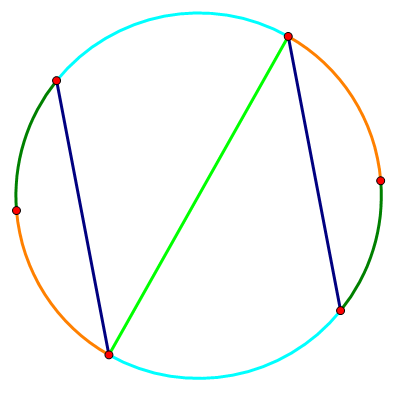
\includegraphics[scale=0.4]{hw13.10.png}}\\
由圖中可以看出 $V=3, E=6, F=4$, 故 Euler-Poincar\'e characteristic = $3-6+4 = 1$.
\end{enumerate}
\end{proof}

%第十二題
\setcounter{theProblemCounter}{11}
\begin{problem}[Ex P283 6.]
Show that $(0,0)$ is an isolated singular point and compute the index at $(0,0)$ of the following vector fields in the plane:
\begin{enumerate}
\item[(a)] $v=(x, y)$.
\item[(b)] $v=(-x,y)$.
\item[(c)] $v=(x,-y)$.
\item[(d)] $v=(x^2-y^2,-2xy)$.
\item[(e)] $v=(x^3-3xy^2,y^3-3x^2y)$.
\end{enumerate}
\end{problem}
\begin{proof}
我們觀察該向量場沿者單位圓繞著原點逆時針旋轉時的轉向,並數其指向 $+x$ 軸方向的次數來計算其 index。\\
在以下各題中, $v=0$ 的解都只有 $(x,y)=(0,0)$, 故 $(0,0)$ 為 isolated singular point.
\begin{enumerate}
\item[(a)]
其轉向為持續逆時針方向且指向 $+x$ 軸方向只有在 $(x,y)=(1,0)$ 時, 故 index=1.\\
\raisebox{1ex-\height}{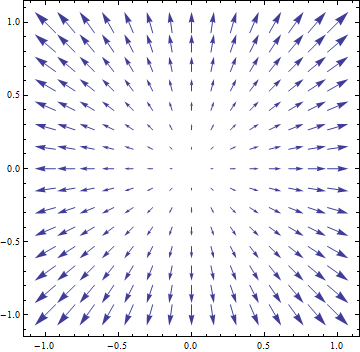
\includegraphics[scale=0.4]{hw13.12.1.png}}
\item[(b)]
其轉向為持續順時針方向且指向 $+x$ 軸方向只有在 $(x,y)=(-1,0)$ 時, 故 index=-1.\\
\raisebox{1ex-\height}{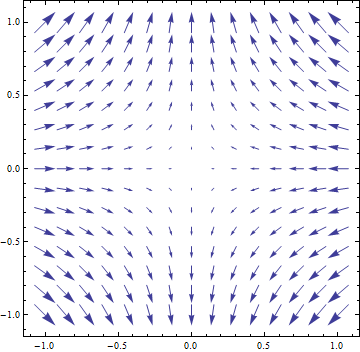
\includegraphics[scale=0.4]{hw13.12.2.png}}
\item[(c)]
其轉向為持續順時針方向且指向 $+x$ 軸方向只有在 $(x,y)=(1,0)$ 時, 故 index=-1.\\
\raisebox{1ex-\height}{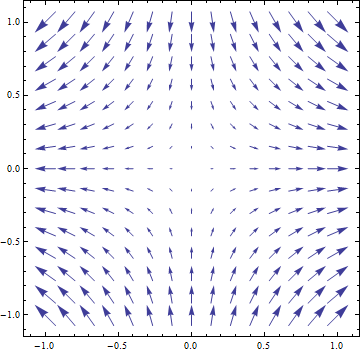
\includegraphics[scale=0.4]{hw13.12.3.png}}
\item[(d)]
其轉向為持續順時針方向且指向 $+x$ 軸方向只有在 $(x,y)=(1,0), (-1,0)$ 時, 故 index=-2.\\
\raisebox{1ex-\height}{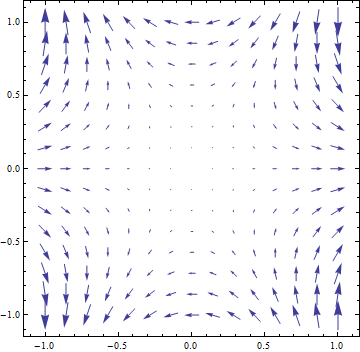
\includegraphics[scale=0.4]{hw13.12.4.png}}
\item[(e)]
其轉向為持續順時針方向且指向 $+x$ 軸方向只有在 $(x,y)=(1,0), (-\frac{1}{2},\frac{\sqrt{3}}{2}), (-\frac{1}{2},-\frac{\sqrt{3}}{2})$ 時, 故 index=-3.\\
\raisebox{1ex-\height}{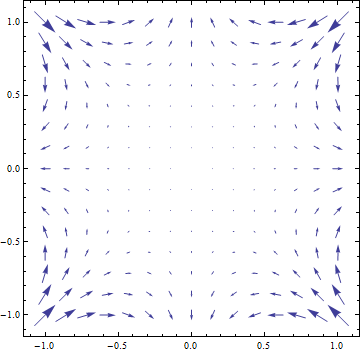
\includegraphics[scale=0.4]{hw13.12.5.png}}
\end{enumerate}
\end{proof}
\end{document}
